% !TeX spellcheck = es_AR
\documentclass[a4paper,spanish,12pt,twoside]{article}
\usepackage{geometry}
\geometry{
	a4paper,
	total={170mm,257mm},
	left=20mm,
	top=20mm,
}
\usepackage[utf8]{inputenc}
\usepackage[spanish,es-tabla]{babel}
\usepackage{graphicx}
\usepackage{caption}
\usepackage{subcaption}
\graphicspath{ {imagenes/} }
\usepackage{amsmath}
\usepackage{graphicx}
\usepackage{wrapfig}
\usepackage{parskip}
\usepackage{listings}
\usepackage[obeyspaces]{url}
\usepackage{caption}
\usepackage{subcaption}
\captionsetup[figure]{name={Figura},labelsep=period}
%\captionsetup[table]{name={Tabla}}
\usepackage{multirow}
\usepackage{multicol}
\usepackage{textcomp} % ° symbol
\usepackage{amsmath}
\usepackage{float} %
\usepackage[hidelinks]{hyperref}
\usepackage[title]{appendix}


\title{Trabajo final de Computación paralela: \textit{tiny molecular dynamics}}
% \footnote no funciona con \maketitle => \thanks
\author{Francisco Fernandez \\ \small{email: \href{mailto:ffernandez@famaf.unc.edu.ar}{ffernandez@famaf.unc.edu.ar}}}
\date{\today}

\begin{document}

\maketitle

\

\

\begin{abstract}

En este trabajo se introducen los conceptos de la dinámica molecular y se presenta un código para un sistema conocido como lo es el de Lennard--Jones. Se realiza una exploración de \path{flags} del compilador \path{gcc} para distintas versiones secuenciales del problema, en las cuales varía la forma de almacenar en memoria las cantidades microscópicas del sistema. Luego se realiza lo mismo observando que secciones del código es capaz de autovectorizar el compilador. Por último se realiza una versión de paralelización con OpenMP y se presenta el scaling del speed-up y la eficiencia en función de la cantidad de hilos para distintos tamaños del problema. El proceso del proyecto puede encontrarse en el repositorio de GitHub\footnote{Directorio de GitHub: \url{https://github.com/fernandezfran/tiny_md}}.%


\end{abstract}

%\end{titlepage}

\section{Introducción teórica al problema}

La dinámica molecular (MD, de sus siglas en inglés, Molecular Dynamics) es una técnica de simulación computacional que considera la interacción entre partículas atómicas para obtener una evolución temporal de las mismas. Esto se logra resolviendo numéricamente las ecuaciones de movimiento de Newton. A partir de cantidades microscópicas (posiciones ($x$), velocidades ($v$), fuerzas ($f$)) se pueden obtener propiedades termodinámicas macroscópicas del sistema en equilibrio (temperatura ($T$), presión ($P$)). Esta técnica tiene aplicaciones en muchas áreas del conocimiento, tales como física, química, biofísica, ciencias de los materiales, etc.

\subsection{Programa de MD}

Una descripción simple de un programa de dinámica molecular se introduce a continuación:

\begin{itemize}
 \item \textit{Inicialización del sistema}: se especifican la cantidad de partículas $N$, la temperatura de referencia $T$ y la densidad $\rho$, de donde puede obtenerse el volumen $V$, largo de la caja $L$. Además, se elije $r_{cut}$ (distancia hasta la cual se considera que las partículas interactúan entre sí), el paso temporal $dt$, las posiciones y velocidades iniciales.
 \item \textit{Cálculo de fuerzas}: se computan las fuerzas sobre todas las partículas.
 \item \textit{Integración de las ecuaciones de movimiento}: se integran las ecuaciones de Newton, con algún integrador que a partir de la condición anterior obtiene las posiciones y velocidades del paso temporal siguiente.
 \item \textit{Mediciones}: se realizan cálculos de distintas cantidades de interés (energía potencial, energía cinética, presión, temperatura).
 \item \textit{Evolución temporal}: al tiempo del sistema se le suma el paso temporal $dt$.
\end{itemize}

A continuación se amplia cada una de estas secciones específicamente para el programa presentado. Ya que hay distintas formas de inicializar el sistema, de calcular las fuerzas con distintos potenciales, algoritmos de evolución, etc.

\subsubsection{Inicialización del sistema}

En este caso las posiciones se inicializan dentro de una red cristalina $FCC$ y las velocidades se dan aleatoriamente entre $-0.5$ y $0.5$, se les resta la velocidad del centro de masa para que el sistema no se esté desplazando y se las multiplica por un factor que involucra la temperatura de referencia.


\subsubsection{Condiciones periódicas de contorno e imagen mínima}

En el caso simulado en este proyecto se utilizan condiciones periódicas de contorno (pbc, periodic boundary conditions), las mismas buscan reproducir un sistema infinito para que no haya efectos de borde y consisten en considerar las $N$ partículas como una celda primitiva de una red infinita de celdas idénticas, en donde, si una partícula sale por un extremo de la caja, ingresa por el opuesto.

\begin{figure}[h]
	\centering
	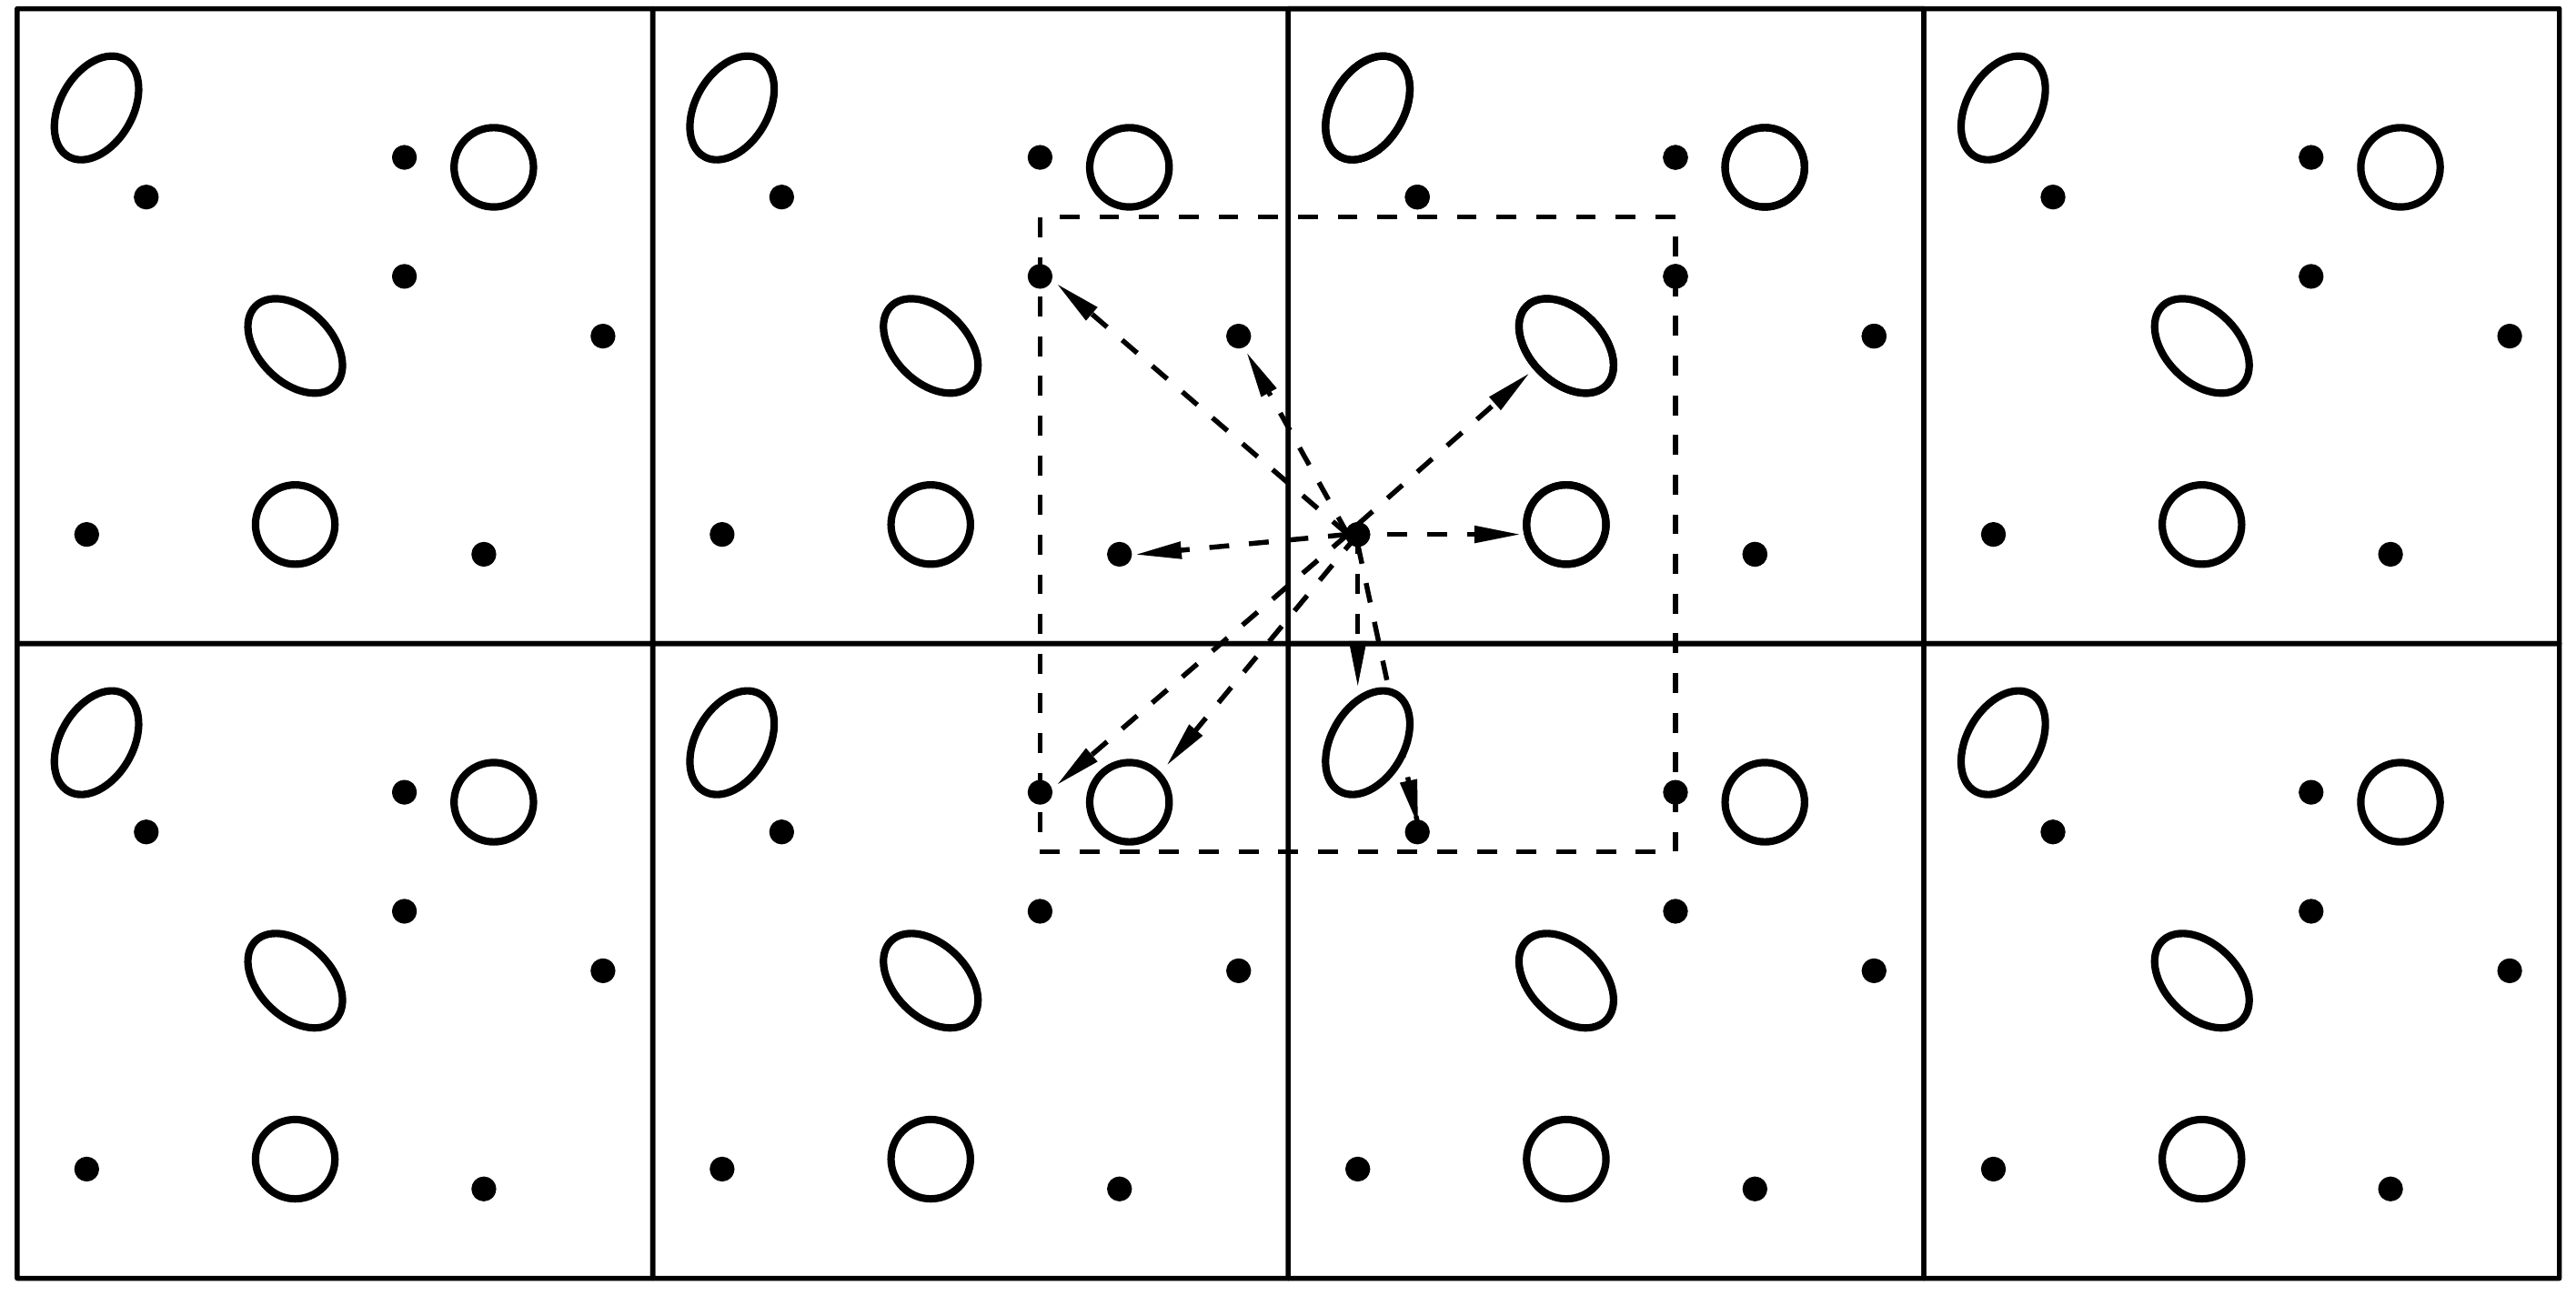
\includegraphics[width=.7\textwidth]{pbc.png}
	\caption{Condiciones periódicas de contorno e imagen mínima.}
	\label{fig:pbc}
\end{figure}

En la figura \ref{fig:pbc} puede verse como se replica una misma celda en todas las direcciones y como al estar centrado en una partícula es necesario salirse de la celda hacia celdas vecinas para encontrar la imagen mínima, que es la distancia más cercana a una partícula.

\subsubsection{Cálculo de fuerzas}

Para el cálculo de las fuerzas se utiliza un potencial aditivo de a pares de Lennard--Jones (12--6), dado por la siguiente expresión,
$$
V_{LJ}(r) = 4\varepsilon \left[ \left( \frac{\sigma}{r} \right)^{12} - \left( \frac{\sigma}{r} \right)^6 \right],
$$
donde $r$ es la distancia entre dos partículas, $\sigma$ es el ``tamaño de la partícula'' y $\varepsilon$ indica que tan profundo es el potencial en el único mínimo que se encuentra en $r_m = 2^{1/6}\sigma$. La forma funcional se muestra en la figura \ref{fig:lj}, si la distancia entre dos pares de partículas es menor a $r_m$ se repelen, si la distancia es mayor, se atraen, y no interactúan si la distancia es infinita (en el caso práctico, mayor a $r_{cut}$).
\begin{figure}[h]
	\centering
	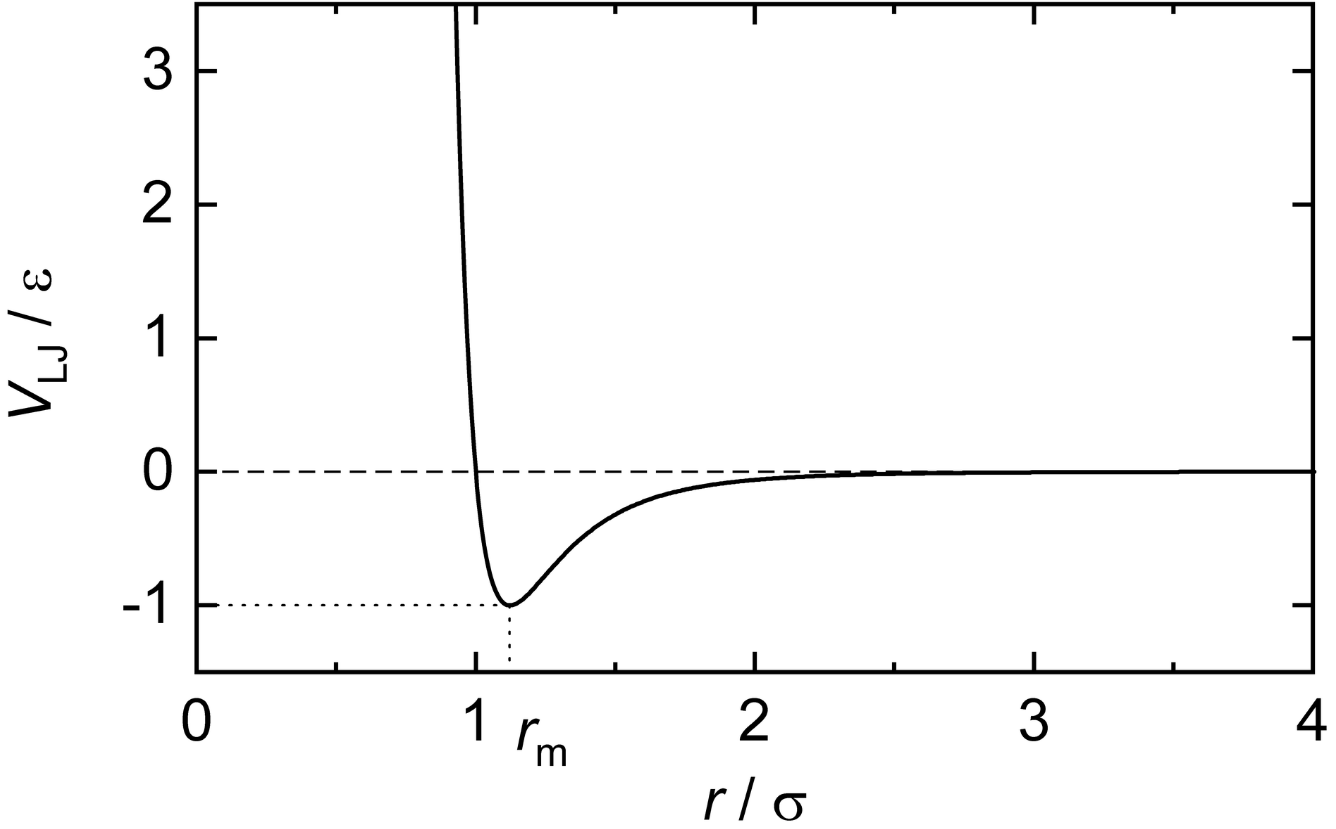
\includegraphics[width=.7\textwidth]{lj.png}
	\caption{Gráfico del potencial de Lennard--Jones.}
	\label{fig:lj}
\end{figure}

Antes de calcular las fuerzas, se necesita la distancia entre dos partículas $i$ y $j$, utilizando la regla de la imagen mínima para considerar la distancia a la imagen más cercana, y calculando la fuerza sólo si dicha distancia es menor a un radio de corte, $r_{cut}$, de la siguiente forma
$$
f_x(r) = -\frac{\partial u(r)}{\partial x} = - \left(\frac{x}{r}\right) \left( \frac{\partial u(r)}{\partial r} \right),
$$
que para el caso del potencial de Lennard--Jones queda
$$
f_x(r) = \frac{24x}{r^2} \left( \frac{2}{r^{12}} - \frac{1}{r^6} \right),
$$
para $y$ y $z$ se tiene una expresión análoga.

Dentro de esta misma sección de código se calcula la energía potencial y la presión instantáneas. 

\subsubsection{Integración de las ecuaciones de movimiento}

Se utiliza el algoritmo \textit{Velocity Verlet}, el mismo conserva la energía total del sistema si se encuentra en el ensamble NVE, que para las posiciones se ve como un desarrollo de Taylor,
$$
r(t + \Delta t) = r(t) + v(t) \Delta t + \frac{f(t)}{2m} \Delta t^2,
$$
y a las velocidades se las actualiza como
$$
v(t + \Delta t) = v(t) + \frac{f(t + \Delta t) + f(t)}{2m} \Delta t,
$$
esto exige calcular las velocidades una vez que se obtuvieron las nuevas posiciones y, a partir de ellas, las nuevas fuerzas.

Aquí se calcula la energía cinética y la temperatura instantáneas.

\subsubsection{Mediciones}

Tanto a la energía potencial como a la presión es necesario sumarles una contribución de cola debido al \textit{truncado y desplazado} que se le realiza al potencial, para que el mismo de anule en $r_{cut}$, esto asumiendo que la energía potencial aportada por una partícula es dominada por las interacciones de las partículas más cercanas. Para la presión se tiene
$$
P_{tail} = \frac{16}{3}\pi\rho^2\varepsilon\sigma^3 \left[ \frac{2}{3}\left( \frac{\sigma}{r_{cut}} \right)^9 - \left( \frac{\sigma}{r_{cut}} \right)^3 \right],
$$
y para la energía
$$
U_{tail} = \frac{16}{3}N\pi\rho\varepsilon\sigma^3 \left[ \frac{2}{3}\left( \frac{\sigma}{r_{cut}} \right)^9 - \left( \frac{\sigma}{r_{cut}} \right)^3 \right].
$$

La presión total será una suma de esta contribución de cola y la presión del virial
$$
P = \rho k_BT + \frac{1}{dV} \left\langle \sum_{i<j} \mathbf{f}(\mathbf{r}_{ij}) \cdot \mathbf{r}_{ij} \right\rangle,
$$
donde $k_B$ es la constante de Boltzmann y $d$ la dimensión del sistema.

La energía potencial total es la suma de la contribución de cola más la suma que se obtiene por la interacción entre las partículas a través del potencial de Lennard--Jones.

Por otro lado, tanto la energía cinética como la temperatura se obtienen utilizando las velocidades de la siguiente manera
$$
E_{kin} = \frac{1}{2} \sum_{i=1}^N m_i v_i^2,
$$
$$
k_BT = \frac{1}{3N} \sum_{i=1}^{N} m_i v_i^2
$$
donde $m_i$ es la masa de la partícula $i$

\subsection{Ecuación de estado}

La ecuación de estado es lo que se obtiene en el programa presentado. La misma relaciona las variables de un sistema bajo ciertas condiciones físicas. En este caso se tiene la presión en función de la densidad del sistema, es decir, se realizan simulaciones en el ensamble canónico (NVT) en las que inicialmente se fija un volumen y la temperatura se mantiene reescaleando las velocidades, para cada una de ellas se calcula la presión para obtener la ecuación de estado $P$ vs $\rho$ que se muestra en la figura \ref{fig:eos}. Para densidades altas el sistema se comporta como un sólido, las posiciones iniciales del cristal FCC se mantienen, y para densidades bajas se comporta como un líquido en el cual las partículas están desorganizadas.

\begin{figure}[h]
	\centering
	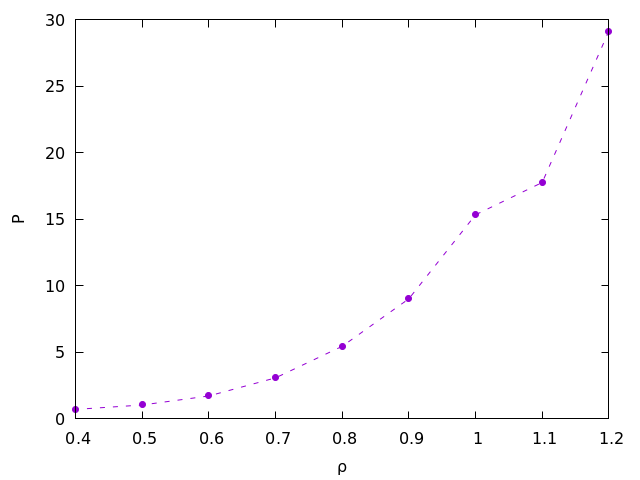
\includegraphics[width=.7\textwidth]{eos.png}
	\caption{Ecuación de estado para la isoterma $T=2.0$.}
	\label{fig:eos}
\end{figure}


\section{Resultados y discusiones}

\subsection*{Unidades y métrica}

Las unidades en las que se encuentran las cantidades físicas dentro del programa son unidades reducidas de Lennard--Jones. Esto quiere decir que se considera $k_B = 1$, que la masa está medida en unidades de $m$, que la distancia está medida en unidades de $\sigma$ y la energía en unidades de $\varepsilon$. A partir de esto se pueden convertir los valores de todas las propiedades físicas, por ejemplo, $T^* = k_BT/\varepsilon$ y $t^* = t \sqrt{\varepsilon/m\sigma^2}$, donde $*$ como superíndice quiere decir que es la forma reducida.

Una métrica usual de dinámica molecular es $ns/day$, es decir, cuántos nanosegundos evoluciona el sistema en un día de simulación. Esta métrica está implementada en el código pero depende del tamaño del problema. En algunas gráficos se presenta la misma, en otras el tiempo total de simulación o el speed-up, definido como
\begin{equation}\label{eq:su}
	S = \frac{tiempo\ original}{tiempo\ nuevo}.
\end{equation}


\subsection*{perf}

En la figura \ref{fig:perf-report} se muestra lo obtenido al realizar \path{perf record ./tiny_md && perf report}. Más del 95\% del tiempo de computo se consume en las funciones \path{forces} y \path{pbc} (que es llamaba por \path{forces} y \path{velocity_verlet}), así que estas son las secciones de código en las que se necesitan hacer optimizaciones.
\begin{figure}[h]
	\centering
	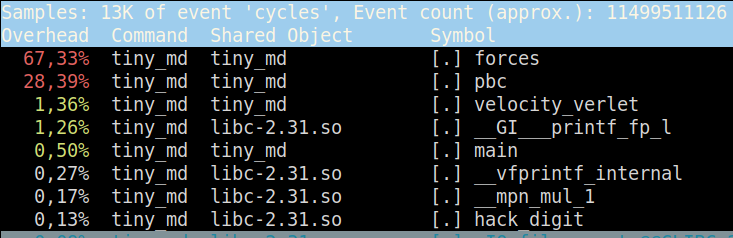
\includegraphics[width=.7\textwidth]{perf-report.png}
	\caption{Porcentaje del tiempo simulado en las funciones del código.}
	\label{fig:perf-report}
\end{figure}

\subsection{Optimizaciones secuenciales}

\subsubsection*{AoS}

Inicialmente en el código las posiciones, velocidades y fuerzas se almacenan en memoria de la forma \textit{Array of Structure}. En el vector de las posiciones (velocidades o fuerzas) se tienen almacenadas en memoria las coordenadas de la misma partícula de forma consecutiva, es decir que, si se lo piensa como matriz, las coordenadas de cada una de las direcciones se encuentran en columnas.

\subsubsection*{SoA}

Esta otra implementación del código cambia la forma del almacenamiento en memoria, aquí como \textit{Structure of Array}. En el vector de las posiciones se tiene primero las coordenadas $x$ de todas las partículas, luego las $y$ y luego las $z$, es decir, que en forma de matriz las coordenadas de cada una de las direcciones están almacenadas en filas.

\subsubsection*{Mixed precision}

En este otro caso en vez de usar \path{double} para los vectores de las posiciones, velocidades y fuerzas, se utilizan \path{float}.

\

En esta parte del trabajo se realizó una exploración con los distintos flags de optimización del compilador \path{gcc} que se encuentran listados en la tabla \ref{tab:os-flags}.
\begin{table}[h]
	\centering
	\caption{Flags de optimización utilizados en el siguiente orden para la obtención de los datos presentados en la figura \ref{fig:os-nsday}.}
	\label{tab:os-flags}
	\begin{tabular}{|r|c|}
		\hline
		& flag \\ \hline
		0 & -O0  \\
		1 & -O1  \\
		2 & -Os  \\
		3 & -O2  \\
		4 & -O3  \\
		5 & -Ofast \\
		6 & -O1 -funroll-loops \\
		7 & -O3 -funroll-loops \\
		8 & -O1 -ffast-math \\
		9 & -O3 -ffast-math \\
		10 & -O1 -funroll-loops -march=native \\
		11 & -O3 -funroll-loops -march=native \\
		12 & -O1 -ffast-math -march=native \\
		13 & -O3 -ffast-math -march=native \\
		14 & -O1 -funroll-loops -ffast-math -march=native \\
		15 & -O3 -funroll-loops -ffast-math -march=native \\
		16 & -O1 -floop-block -floop-interchange \\
		17 & -O3 -floop-block -floop-interchange \\
		18 & -O1 -funroll-loops -floop-block -floop-interchange -march=native \\
		19 & -O3 -funroll-loops -floop-block -floop-interchange -march=native \\
		\hline
	\end{tabular}
\end{table}
Las mediciones se realizaron en \path{zx81}, ver Apéndice \ref{app:zx81}, utilizando \path{SLURM}, scripts de \path{python3} y \path{perf stat}. Los resultados obtenidos, para un sistema con $N=256$ partículas, se muestran en la figura \ref{fig:os-nsday}, donde se gráfica los $ns/day$ en función de los distintos flags de optimización para las tres versiones del programa explicadas anteriormente.


\begin{figure}[h]
	\centering
	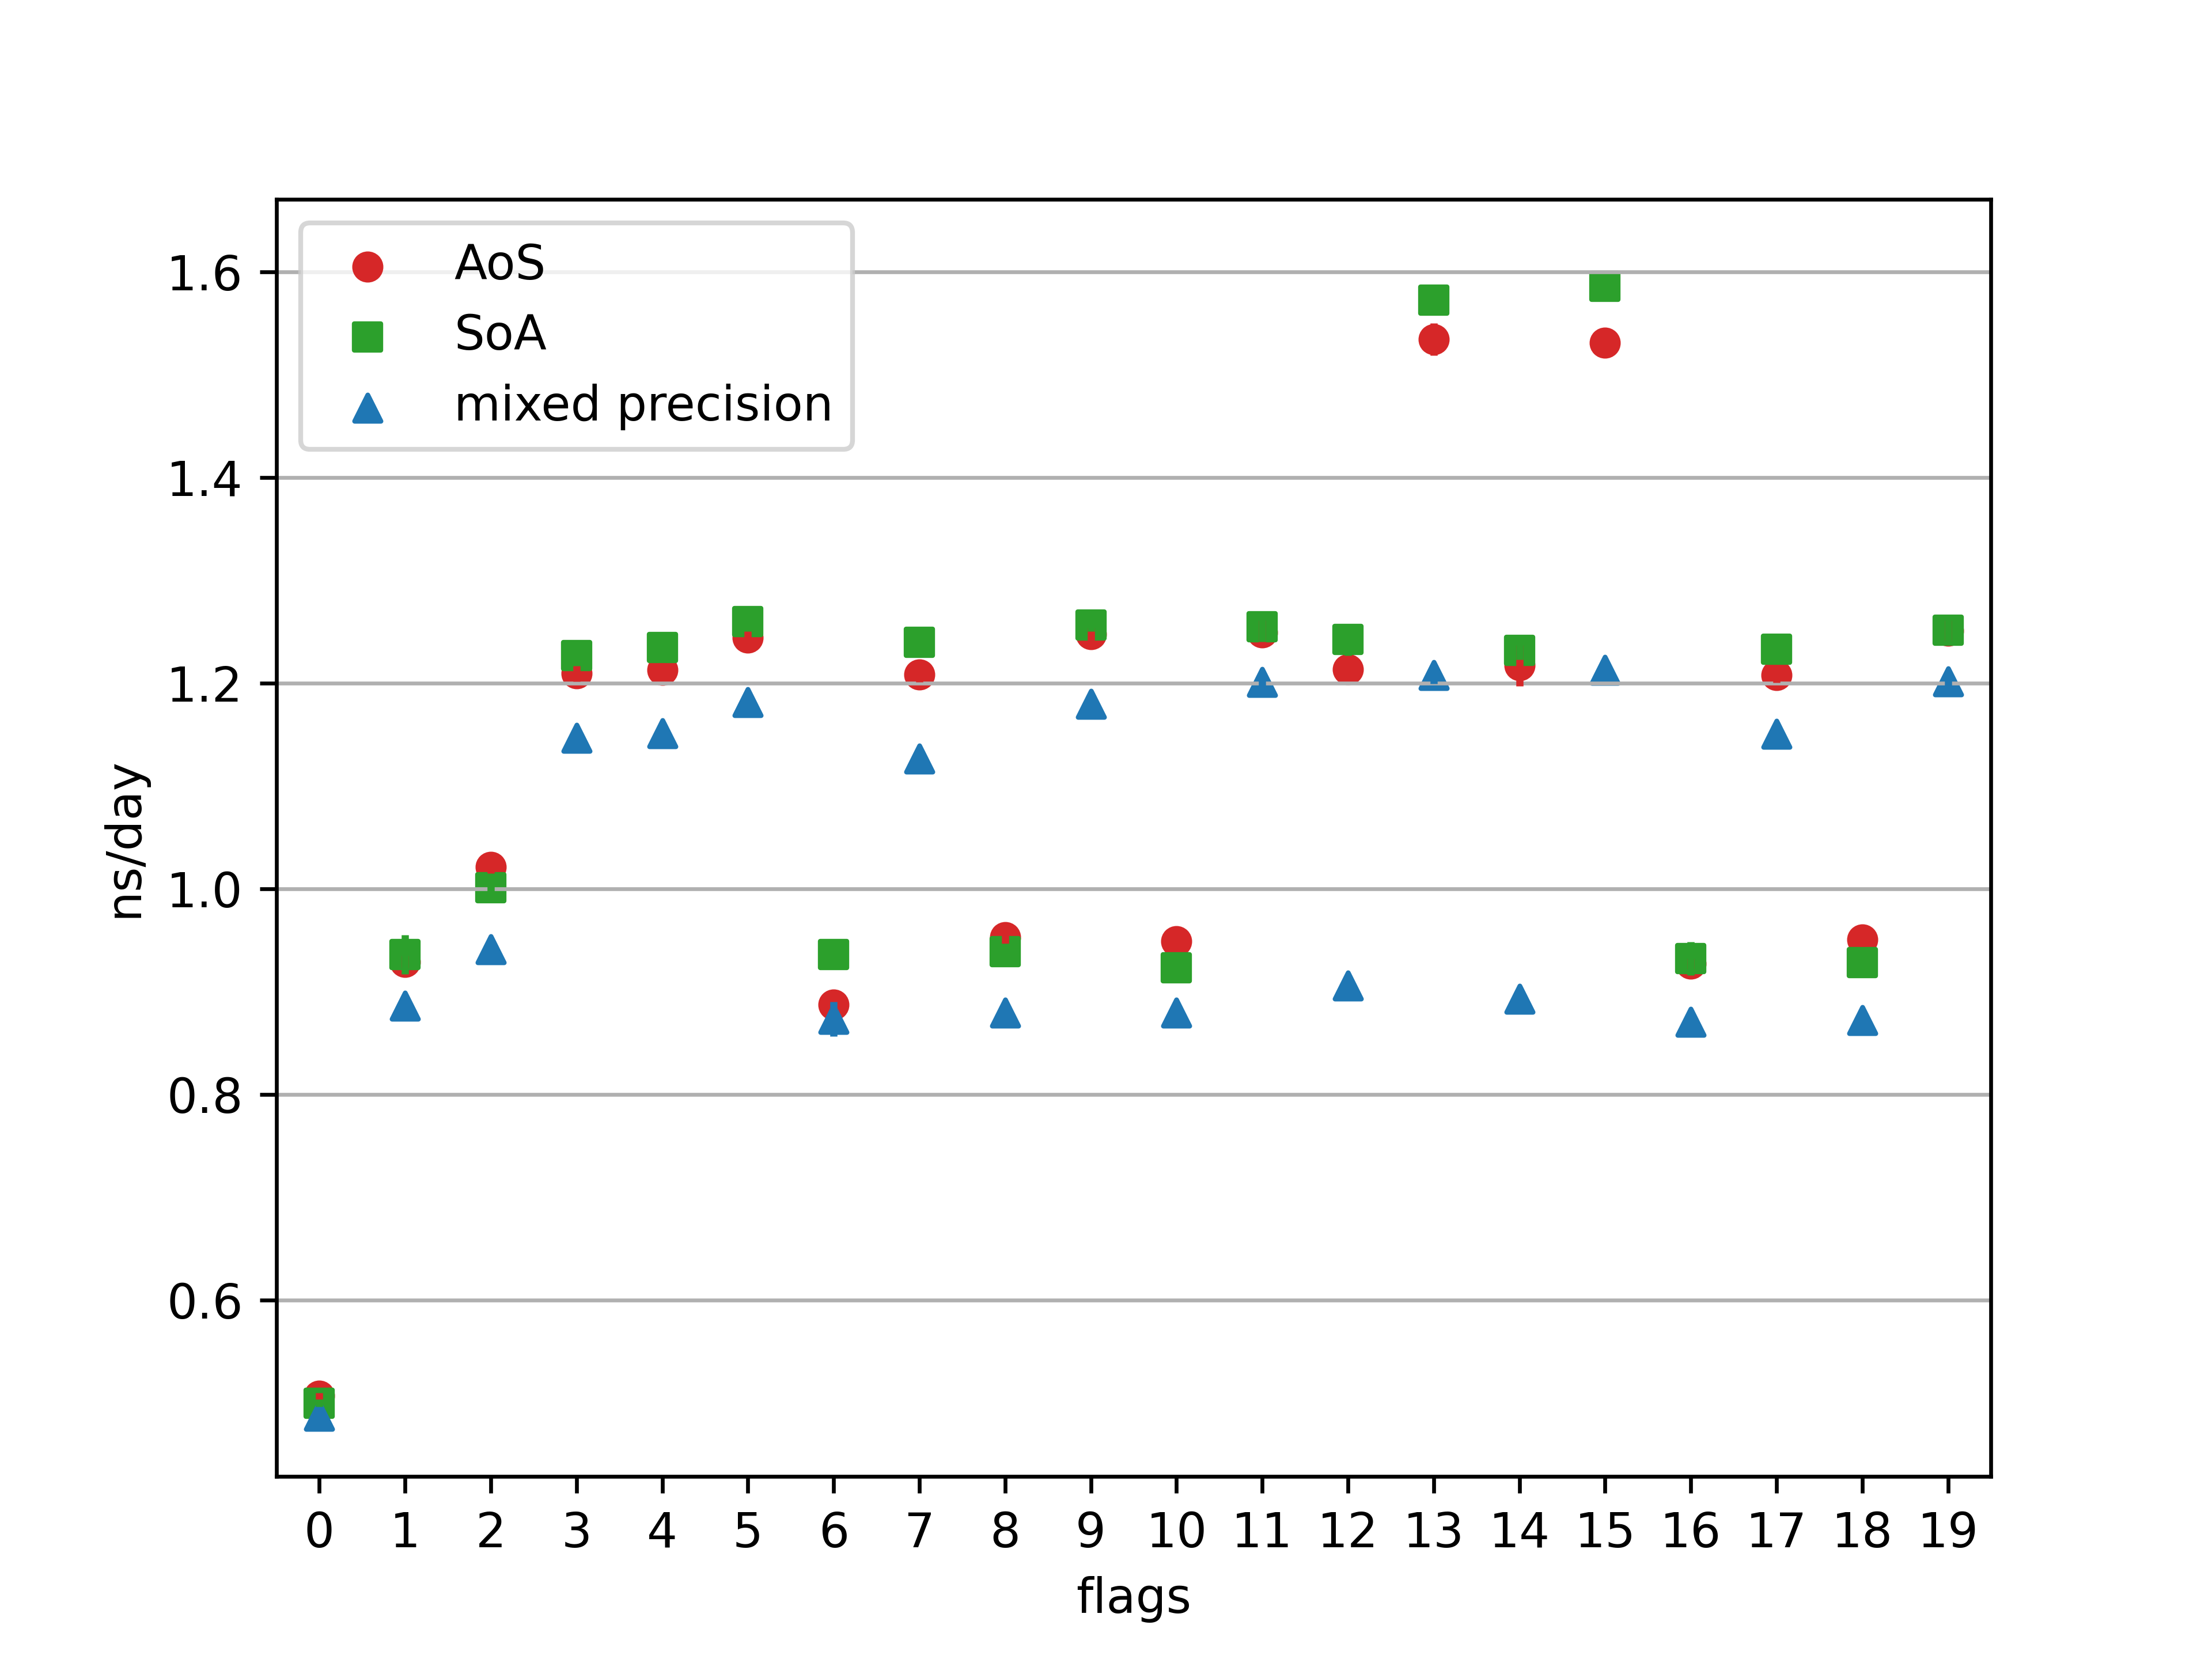
\includegraphics[width=.8\textwidth]{1-o_s-nsday.png}
	\caption{Métrica $ns/day$ para los distintos flags de optimización listados en la tabla \ref{tab:os-flags}. Para la obtención de cada punto se realizaron 30 mediciones y el número de partículas fue $N = 256$. Las barras de error en cada punto son menores que el tamaño del mismo.}
	\label{fig:os-nsday}
\end{figure}
Lo que se observa en la figura \ref{fig:os-nsday} es que para la versión SoA se obtienen resultados ligeramente mejores que para la AoS y que la versión mixed precision tiene menor performance que las otras dos. Para los tres casos puede afirmarse, debido a que las barras de error son menores al tamaño de los puntos, que la combinación de flags que mejor resultados da es \path{-O3 -funroll-loops -ffast-math -march=native}. De la cual se obtiene $(1.60 \pm 0.02)\ ns/day$ para la versión SoA. Inicialmente se tenía $(0.500 \pm 0.003)\ ns/day$, lo que da un speed-up de 3.2x.



\subsection{Vectorización}

\subsubsection*{Autovectorización}

Se utilizó el flag de autovectorización, \path{-ftree-vectorize}, en la misma búsqueda de la tabla \ref{tab:os-flags}. Además de las versiones AoS y SoA, se agregó una versión \textit{Naive--loops}, a partir de la versión SoA, en la cual se juntan las operaciones que se hacen en $x$, $y$, $z$ dentro de un loop que va de $0$ a $2$, en todas las partes del código en las que fue posible. Se presentan los datos obtenidos para la mejor combinación de flags en la tabla \ref{tab:autovec}. Tanto para AoS como para SoA la mejor combinación sigue siendo la encontrada anteriormente, para \textit{Naive--loops} se obtuvo que la mejor es \path{-O1 -funroll-loops -ffast-math -march=native -ftree-vectorize}, que da, comparando con el proyecto inicial, un speed-up de 3.46x.
\begin{table}[h]
	\centering
	\caption{Resultados de la autovectorización en ns/day, se realizaron 10 mediciones para dar cada uno de los valores.}
	\label{tab:autovec}
	\begin{tabular}{|l|c|}
		\hline
	    versión  	& ns/day           \\
	    \hline
		AoS         & $1.55 \pm 0.02$  \\ 
		SoA         & $1.577 \pm 0.004$  \\
		naive loops & $1.73 \pm 0.01$  \\
		\hline
	\end{tabular}
\end{table}

Utilizando el flag de compilación \path{-fopt-info-vec-optimized} se ve que tanto para AoS como para SoA los loops autovectorizados son básicamente los mismos, parte de la inicialización de las velocidades, el reescaleo de las mismas y \path{velocity_verlet}. Como se aprecia en los datos mostrados en la tabla \ref{tab:autovec}, estas optimizaciones no son significativas en la simulación con respecto al laboratorio anterior. Por otro lado, en la versión \textit{Naive--loops} no se optimiza \path{velocity_verlet} pero sí \path{pbc} y parte de \path{forces} (el loop más interno y el cálculo de la distancia, pero no el de la fuerza y el cargado de estos datos al vector).

\subsubsection*{SSE}
No me estaría saliendo la condición del if en el computo de las fuerzas...


\subsection{Paralelización: OpenMP}

Al computar las fuerzas en cualquiera de las versiones secuenciales del programa, se utiliza que la fuerza que siente la partícula $i$ por causa de la partícula $j$ es igual, pero con signo opuesto, a la que siente la partícula $j$ por la $i$. Es decir, no es necesario recorrer la matriz completa para calcular todas las fuerzas, si no que se recorre la triangular superior (o inferior) y con eso alcanza para completar la triangular inferior (o superior).

En el caso paralelo sólo se pueden cargar a los vectores los valores de las fuerzas de las partículas $i$ que se están recorriendo en el hilo correspondiente, ya que el resto de la matriz está en el resto de los hilos. Por lo cual, en la versión paralela se realizan más operaciones que en la secuencial.

En la sección del código que calcula las fuerzas se realizó un schedule manual por hilo y se colocó el decorador \path{#pragma omp parallel} declarando las variables compartidas por default y especificando cuales son las privadas del hilo (que se declararon antes del decorador). Además se agregó \path{reduction(+:pot,pres_vir)} para realizar la suma paralela de la energía potencial y del virial de la presión.

La métrica utilizada hasta ahora (ns/day) es la usual en dinámica molecular, pero es dependiente del tamaño del problema. Por eso, para comparar distintos tamaños en función de la cantidad de hilos en OpenMP se opta por presentar el tiempo de simulación, el speed-up, definido en la ecuación \ref{eq:su}, y la eficiencia,
$$
E = \frac{S}{N},
$$
donde $S$ es el speed-up y $N$ es el número de hilos.

\begin{figure}[h]
	\centering
	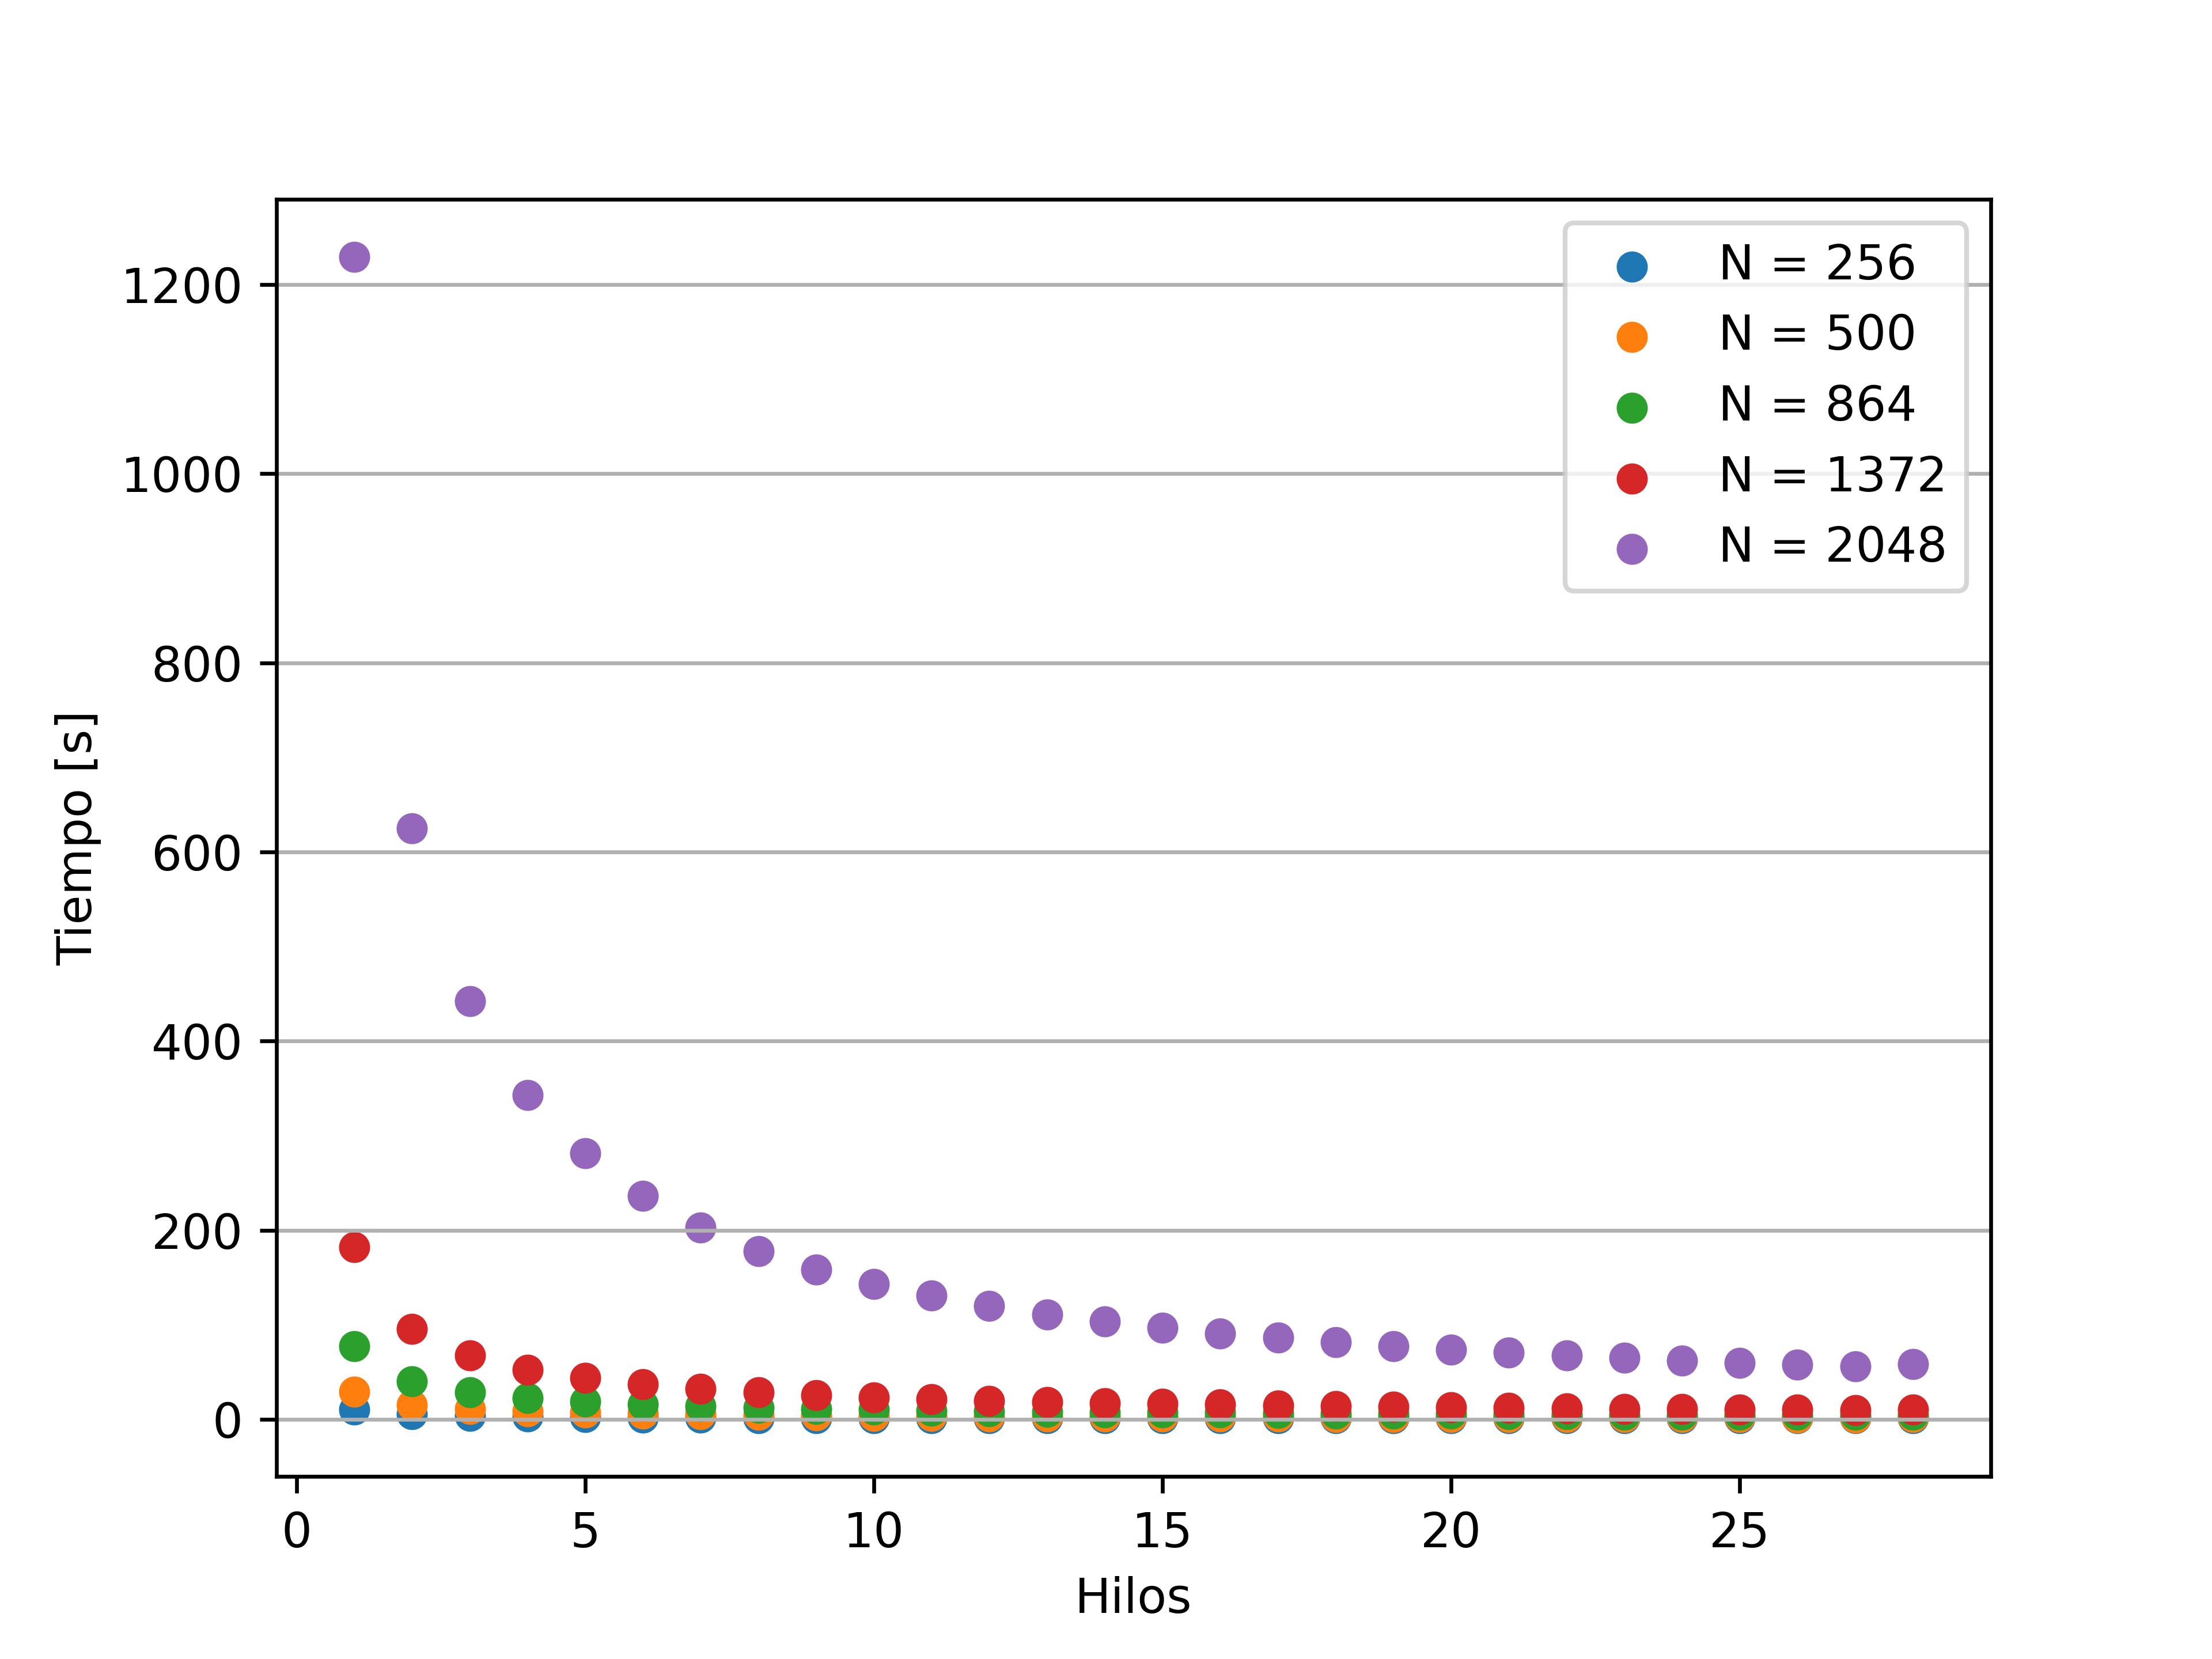
\includegraphics[width=.8\textwidth]{3-omp-tiempo.png}
	\caption{Tiempo de simulación en función de la cantidad de hilos de OpenMP para distintos tamaños del problema.}\label{fig:omp-tiempo}
\end{figure}
En la figura \ref{fig:omp-tiempo} se muestran los resultados obtenidos para el tiempo de simulación en función de la cantidad de hilos de OpenMP para distinta cantidad de partículas. Los resultados fueron obtenidos utilizando \path{OMP_PROC_BIND=ture OMP_NUM_TRHEADS=i perf stat -r 10 ./tiny_md}, donde la primera opción hace que los hilos de OpenMP queden fijos en un sólo hilo físico y en la segunda opción se puede ir variando la cantidad de hilos $i$ que se toman. Se optó por bajar la cantidad de mediciones con respecto a las mediciones anteriores para obtener resultados para problemas más grandes en un tiempo de cómputo razonable.
La tendencia es la esperada, a mayor cantidad de hilos se tiene que el problema corre más rápido y que, por ejemplo, utilizando 8 hilos se puede correr un problema de $N = 2048$ a la misma velocidad que se correría en un sólo hilo un problema de $N = 1372$, que es un poco más que la mitad de la cantidad de partículas.

\begin{figure}[h!]
	\centering
	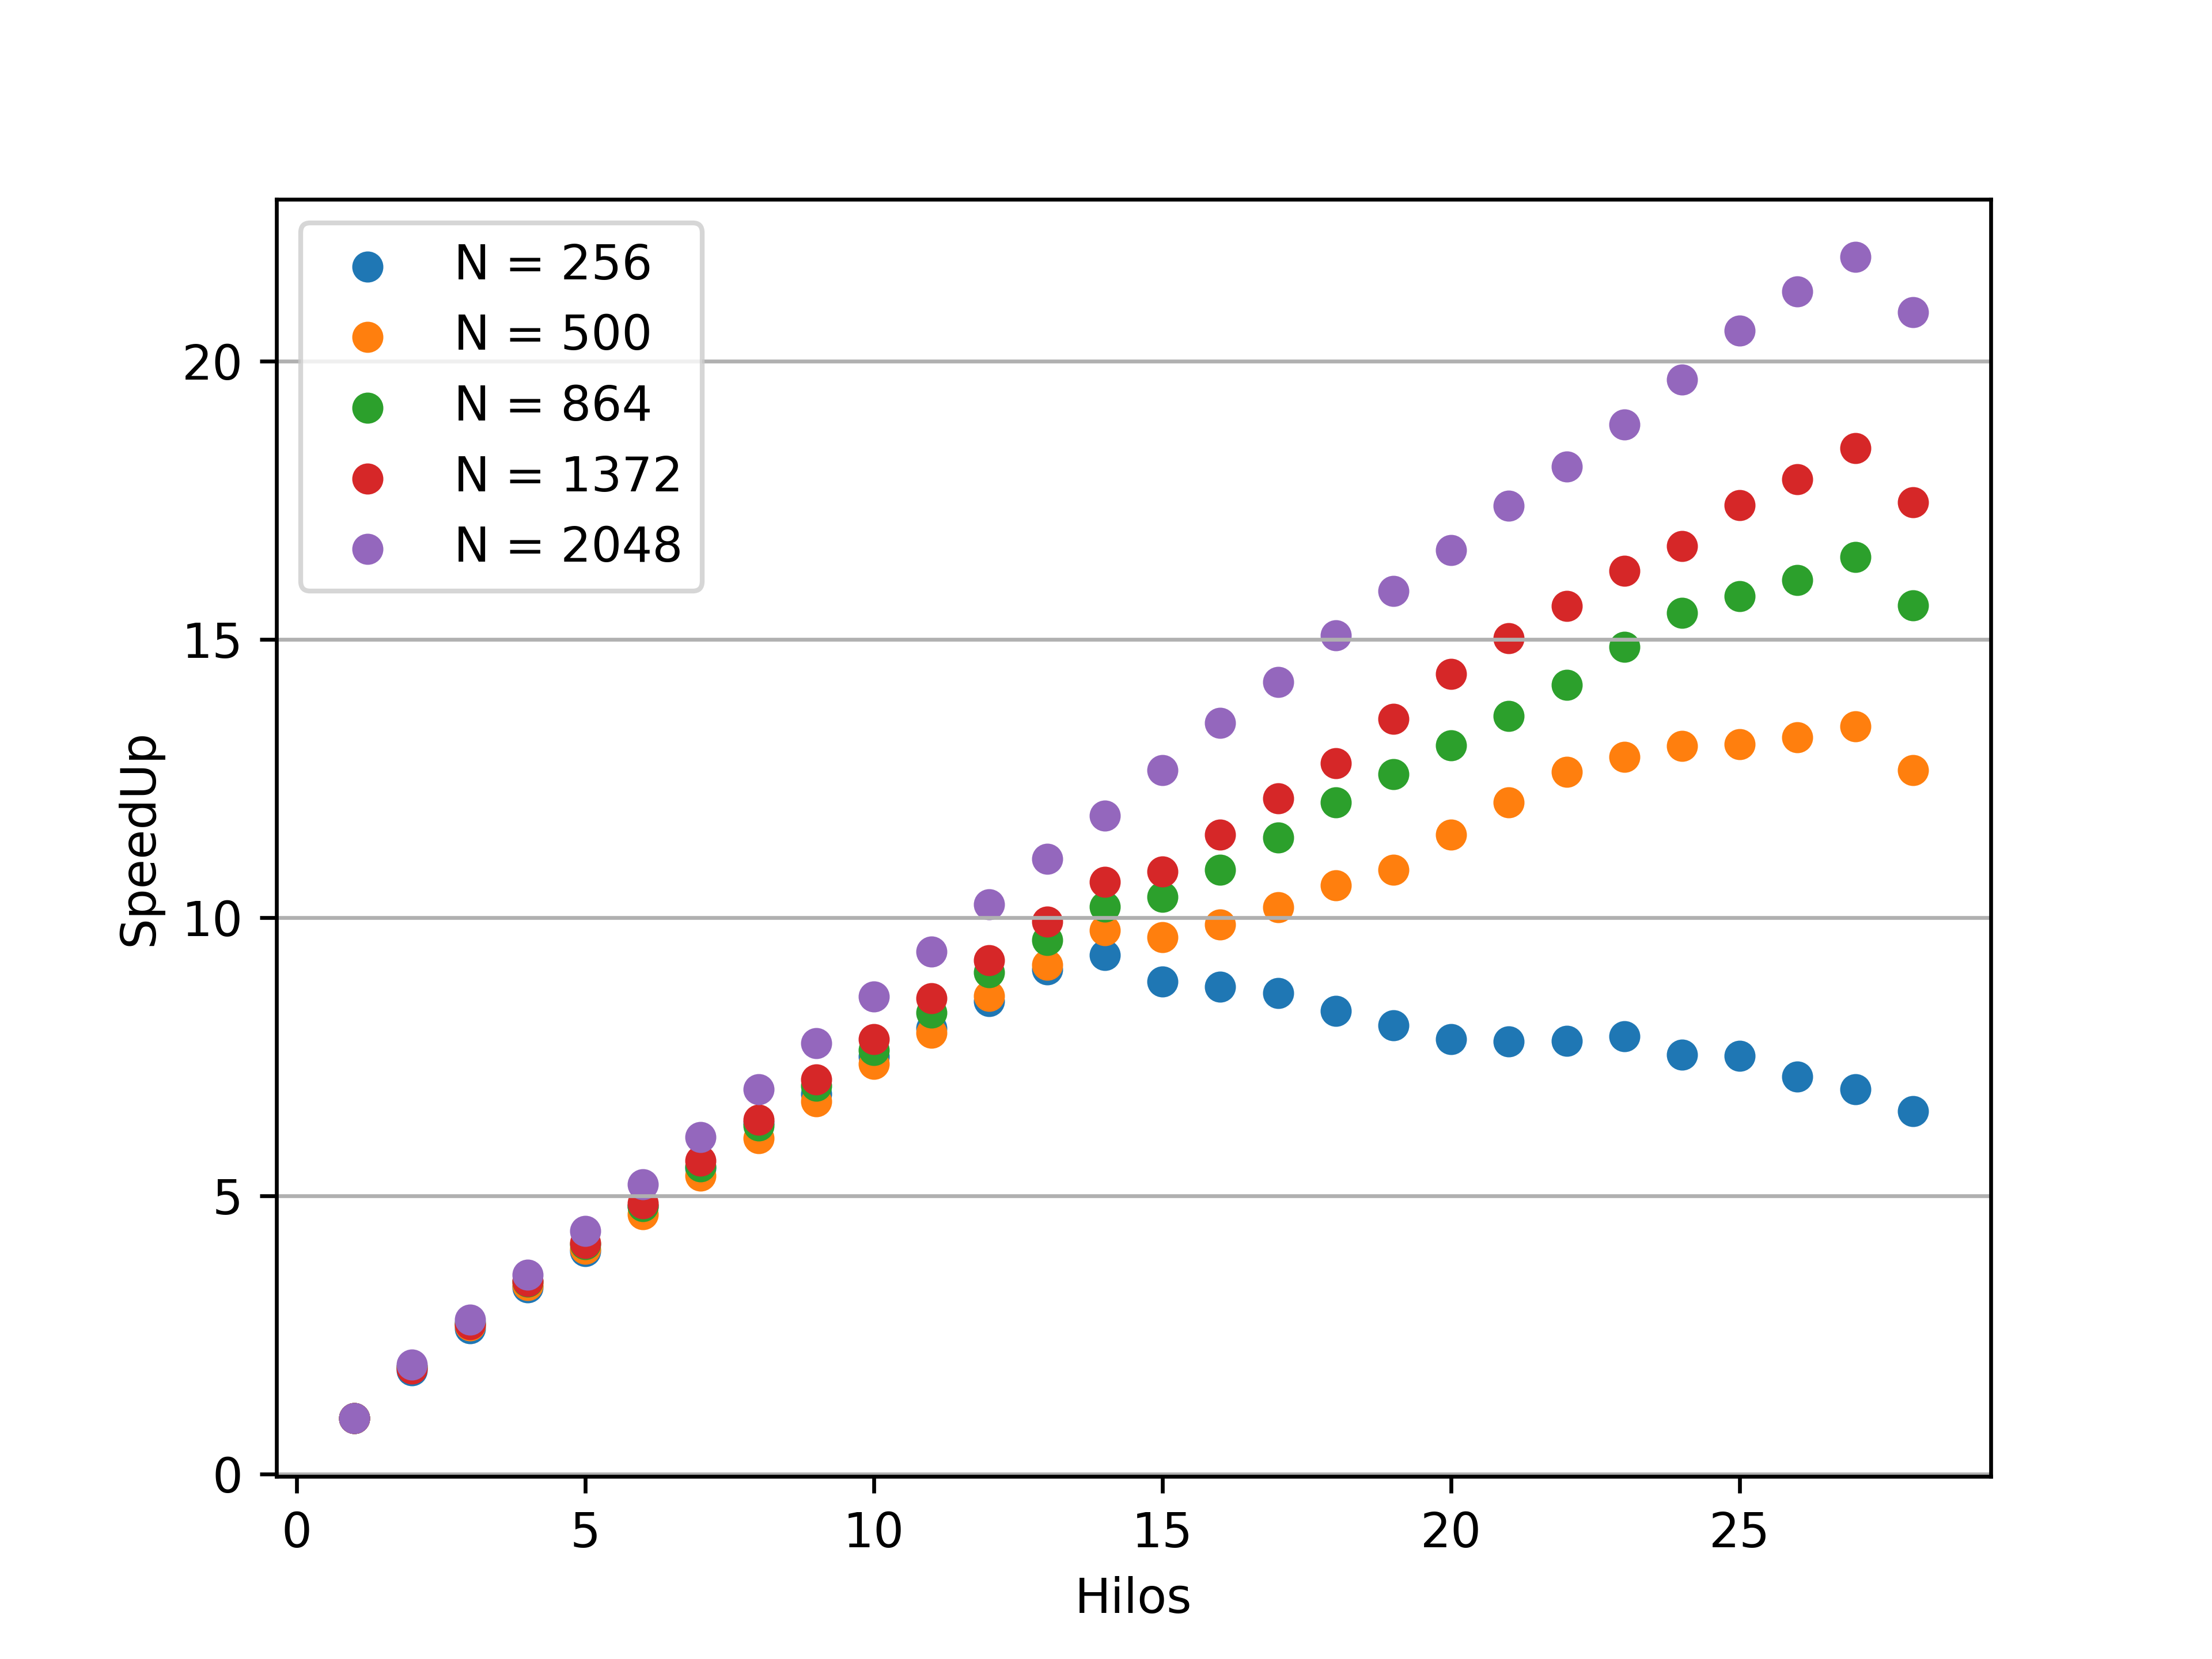
\includegraphics[width=.8\textwidth]{3-omp-speedup.png}
	\caption{Speed up en función de la cantidad de hilos de OpenMP para distintos tamaños del problema.}\label{fig:omp-speedup}
\end{figure}
También se presenta el speed-up en función de la cantidad de hilos en la figurad \ref{fig:omp-speedup}, calculado a partir de los datos presentados. Para un tamaño muy chico del problema ($N=256$) se ve como el speed up aumenta de manera lineal sólo hasta $14$ hilos, que es donde termina un \textit{numa node} y luego empieza el otro y ya no es conveniente seguir agregando hilos, ya que el speed up empieza a disminuir. Para un tamaño de problema chico ($N=500$) se tiene que el speed up es siempre creciente, pero la pendiente es mayor en los primeros $14$ hilos que en los siguientes. Este efecto que ocurre a partir del hilo número $15$ puede deberse a la comunicación entre los hilos a través del nodo. Para un tamaños medianos del problema ($N=864$ y $N=1372$) este efecto es menos notable ya que cada hilo empieza a tener más partículas que computar. Finalmente, para un tamaño grande ($N = 2048$), se tiene que el speed up es lineal, salvo por el último punto que decae cuando todos los hilos están prendidos.

Por último, se muestra la eficiencia en función de la cantidad de hilos de OpenMP para distintos tamaños del problema en la figura \ref{fig:omp-eficiencia}. Se observa que para $N = 2048$ la eficiencia decae lentamente de un $90$\% a un $80$\%, exceptuando el último punto. Para el resto de los casos se ve como la eficiencia decae hasta un $70$-$80$\%, hasta el \textit{numa node}. Después del hilo número $15$, para $N = 1372$, la eficiencia se mantiene al rededor del $70$\%, mientras que para $N = 864$ decae del $70$\% al $60$\%. Para $N=500$ la eficiencia decae del $60$\% al $50$\% y para $N=256$ se pierde rápidamente, encontrándose por debajo del $50$\% y llegando a ser cercana al $20$\%.
\begin{figure}[h]
	\centering
	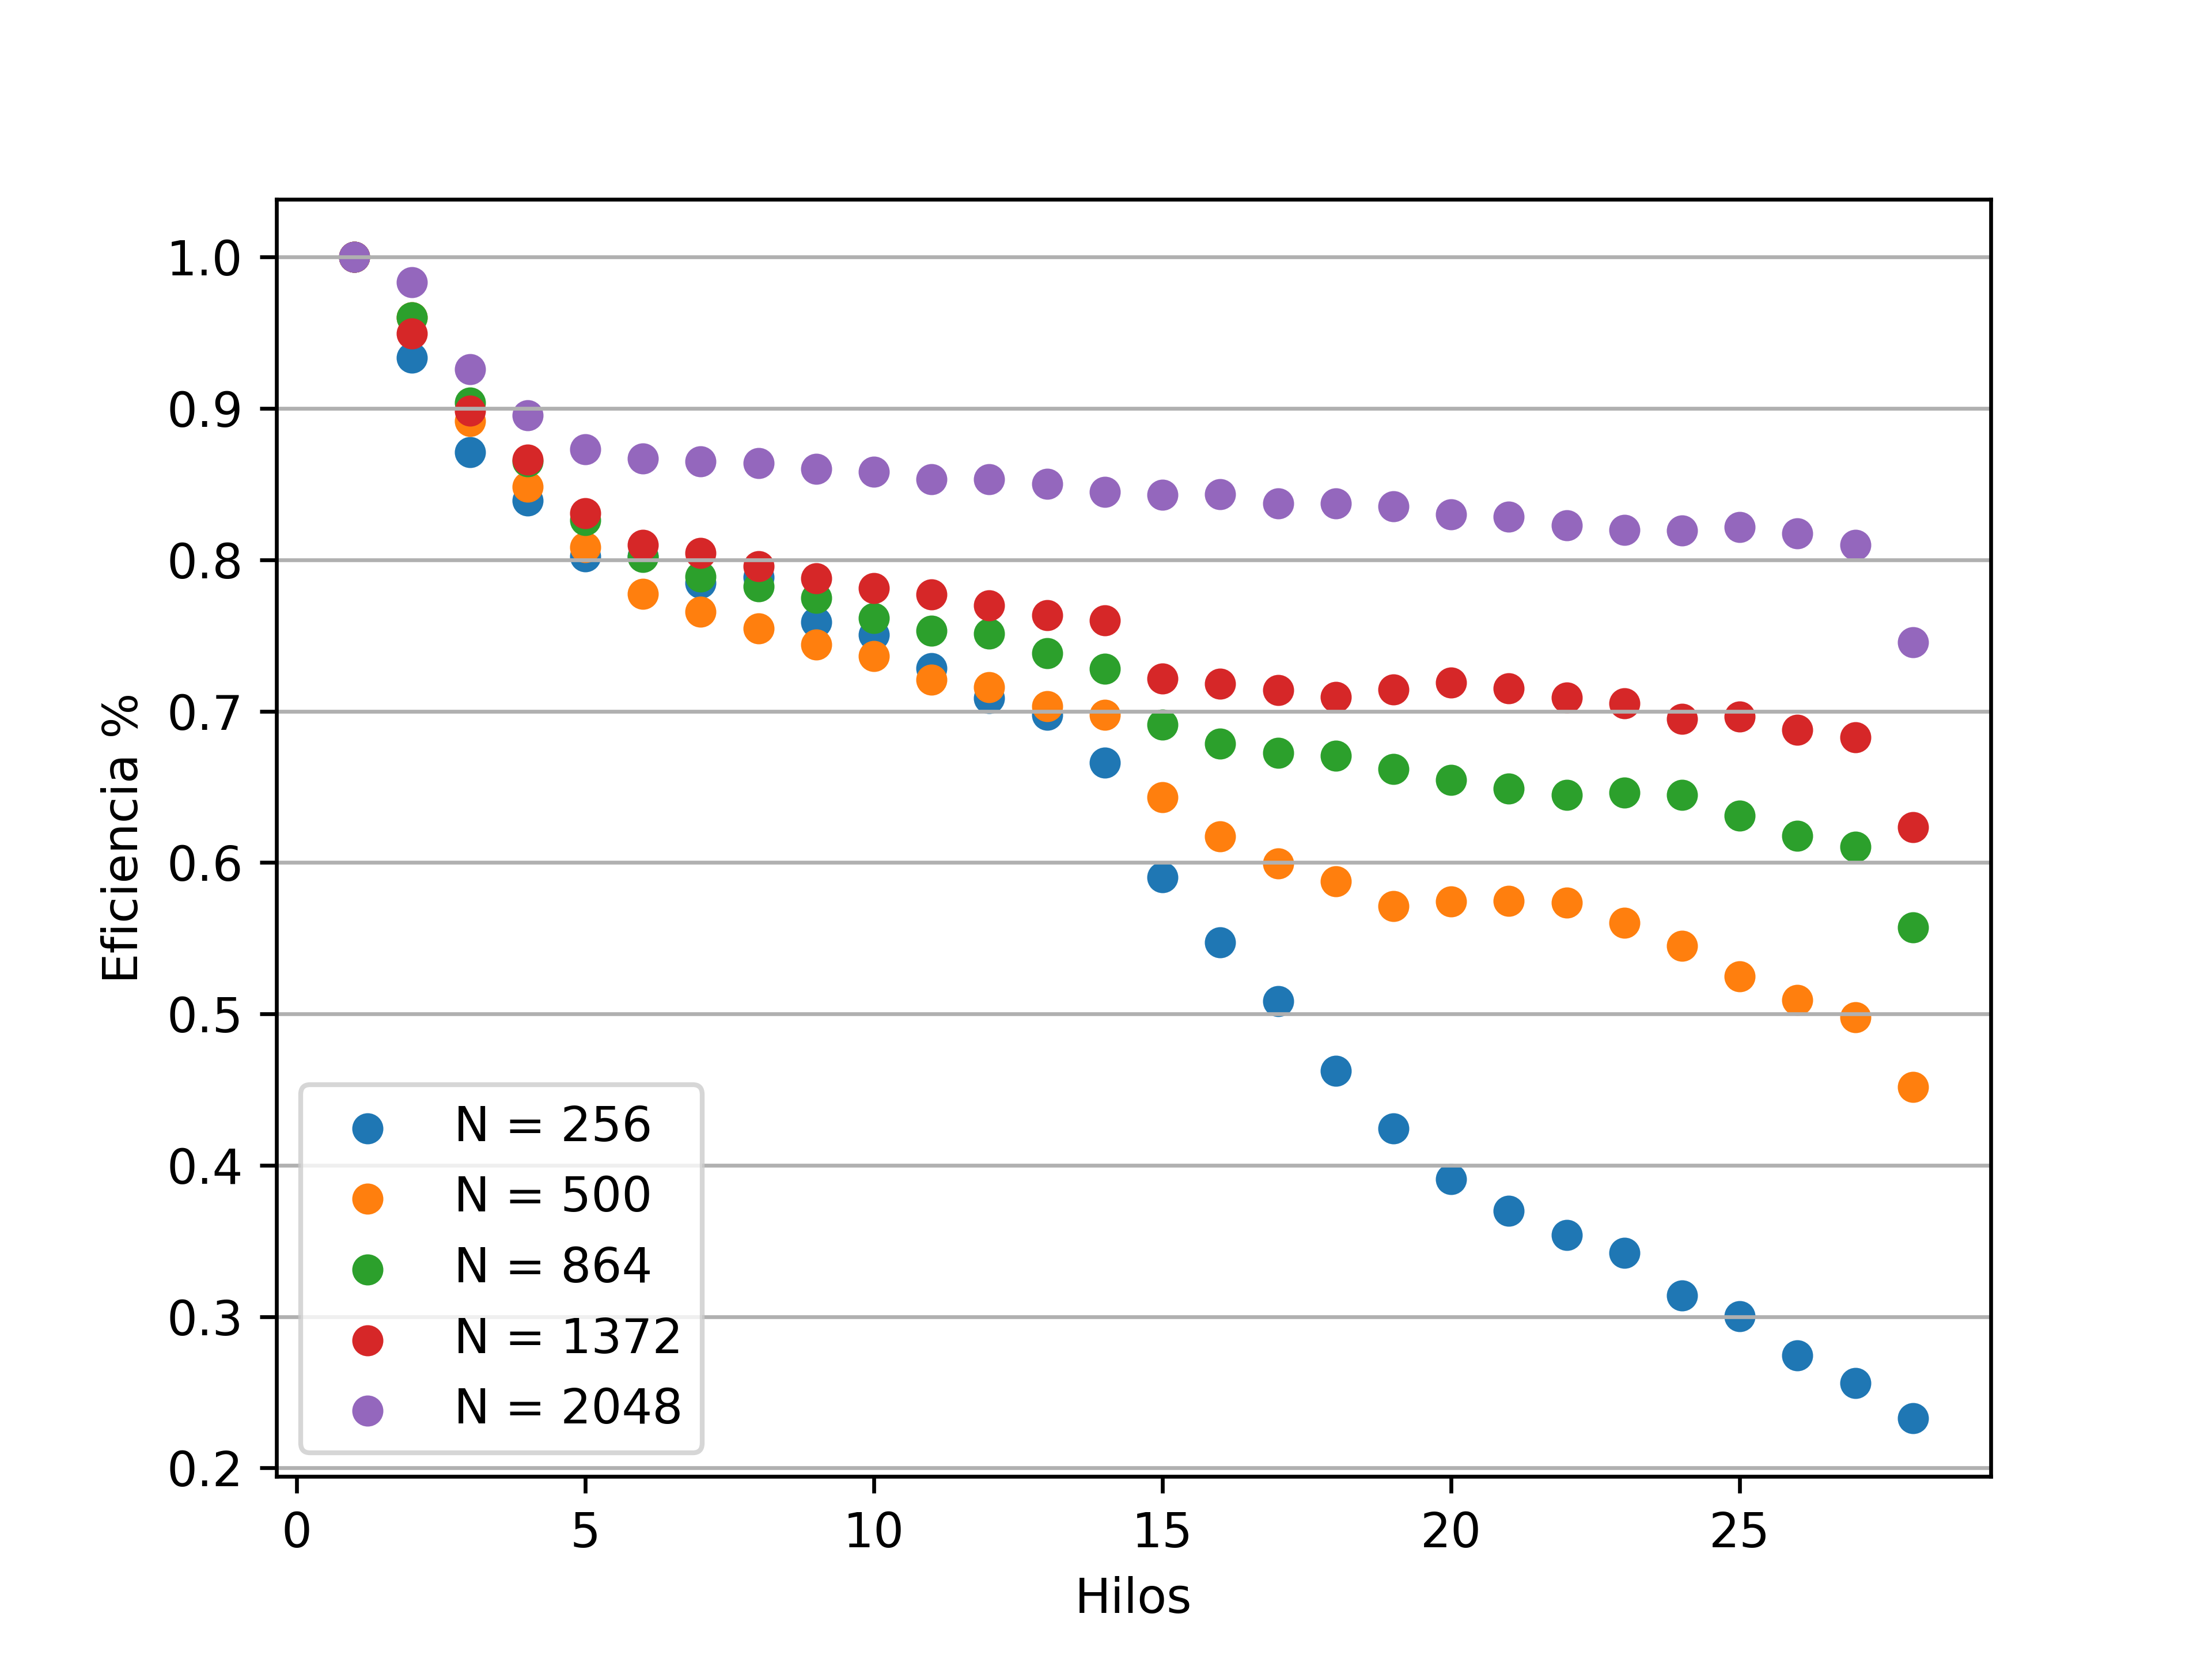
\includegraphics[width=.8\textwidth]{3-omp-eficiencia.png}
	\caption{Eficiencia en función de la cantidad de hilos de OpenMP para distintos tamaños del problema.}\label{fig:omp-eficiencia}
\end{figure}

\clearpage
\pagebreak

\begin{appendices}
	\section{zx81}\label{app:zx81}
	Características de \path{zx81}:
	\begin{itemize}
		\item Intel(R) Xeon(R) CPU E5-2680 v4 @ 2.4GHz.
		\item Memoria cache:
		\begin{itemize}
			\item L1d: 896 KiB
			\item L1i: 896 KiB
			\item L2: 7 MB
			\item L3: 70 MB
		\end{itemize}
		\item 128 GiB de RAM DDR4.
		\item Debian 5.10.9-1 (2021-01-20) x86\_64 (GNU/Linux).
	\end{itemize}
\end{appendices}


\end{document}